\documentclass[11pt]{article}

\usepackage[a4paper,margin=1in]{geometry}
\usepackage{amsmath,amssymb,amsthm,mathtools}
\usepackage{bm}
\usepackage{enumitem}
\usepackage[colorlinks=true,linkcolor=blue,citecolor=blue,urlcolor=blue]{hyperref}
\usepackage[nameinlink,capitalise]{cleveref}

\usepackage[backend=biber,style=alphabetic]{biblatex}
\addbibresource{dan.bib}

\allowdisplaybreaks

\title{Backpressure Entanglement Swapping in \\ Quantum Networks}
%\author{Javad Ghaderi}
\date{\today}

\newtheorem{theorem}{Theorem}
\newtheorem{lemma}{Lemma}
\newtheorem{definition}{Definition}
\newtheorem{remark}{Remark}

\newcommand{\E}{\mathbb{E}}
\newcommand{\Ncal}{\mathcal{N}}
\newcommand{\Pairs}{\mathcal{P}} % unordered pairs x<y

\newcommand{\Javad}[1]{\textcolor{red}{JG: #1}}

\begin{document}
\maketitle

\begin{abstract}
One of the main uses of the Quantum Internet will be, through swaps at repeaters, to establish entangled Bell Pairs between geographically distributed pairs of nodes that require their consumption to perform distributed quantum computations.  Depending on the geographic locations of the nodes and the geographic placement of the repeaters, some consumption requests that are ``closer together'' are more easily satisfied than others.  In environments where Bell Pair generation is a sufficient but limiting resource to meet this consumption demand, policies that do not explicitly account for the existing consumption demand can be unstable, meaning they can starve those consumption requests that are relatively harder to satisfy.  
%
We consider the recently proposed path-oblivious approach to Bell Pair distribution that advocates for swapping Bell Pairs throughout the network proactively, as opposed to waiting for explicit consumption requests to swap.  While prior art showed via a linear programming formulation that in theory, path-oblivious strategies exist that are stable, in that they can meet any feasible consumption demand, no practical distributed algorithm has yet been presented that can provably accomplish this feat.  In this paper, we begin by showing that a prior ``max-min'' based algorithm that does not explicitly consider consumption requests can fail to stable in settings where stable solutions exist.  Our main result is to derive a backpressure-based distributed algorithm which we prove achieves stability when stable solutions exist.  We also perform a preliminary exploration of the effects of limiting communication between nodes of their state needed by swapping algorithms to make informed swapping choices, and show that our backpressure-based mechanism can maintain its stability guarantees even when such communication is limited.


%We consider a quantum network where Bell pairs $[x,y]$ can be generated on certain links and can be moved across the network via entanglement swapping. Each node $i$ can perform at most $K_i$ swaps per time slot. Consumption requests arrive between end nodes $(x,y)$ at rates $\lambda_{xy}$, and must be served by consuming Bell pairs $[x,y]$. We propose a fully distributed backpressure rule for entanglement swapping. The rule is structured using two queues for each pair $(x,y)$: $\gamma_{xy}(t)$ (demand pressure) and $\alpha_{xy}(t)$ (Bell pair scarcity pressure). At each node $i$, the algorithm schedules up to $K_i$ swaps with the largest positive ``pressure differences'' $W_i(y,y')
%:= \alpha_{yy'}-\alpha_{iy}-\alpha_{iy'}$, and serves demand on pair $(x,y)$ if $\gamma_{xy}\ge\alpha_{xy}$. We show (i) how these queues and the swap rule arise from the dual of a feasibility Linear Program (LP), and (ii) how a quadratic Lyapunov fucntion on $(\gamma,\alpha)$ certifies stability under any offered load $\lambda$ strictly inside the capacity region. Extensive simulation results are presented to show the performance of the proposed algorithm compared to other baselines. 
\end{abstract}


\section{Intro}

\begin{itemize}

\item Main use of quantum Internet: distribute Bell Pairs to where they are needed.  Possibly geographically diverse

\item Large bodies of work have considered what are called \em{planned-path} approaches, 
\end{itemize}
\section{Network model}

\subsection{Exogenous consumption and generation processes.} Let $\Ncal$ be a finite node set. Let
\[
\Pairs \;:=\; \{\, xy : x,y\in\Ncal,\ x<y \,\}
\]
denote unordered distinct node pairs (we write $xy$ for $(x,y)$). For each $xy\in\Pairs$:

\begin{itemize}[leftmargin=2em]
\item $A_{xy}(t)\in\mathbb{Z}_{\ge 0}$ is the number of consumption \emph{requests} arriving in slot $t$ that require consuming a Bell pair $[x,y]$. We assume $\E[A_{xy}(t)]=\lambda_{xy}$ and that $\{A_{xy}(t)\}$ have uniformly bounded second moments.
\item $G_{xy}(t)\in\mathbb{Z}_{\ge 0}$ is the number of Bell pairs $[x,y]$ \emph{directly generated} in slot $t$ (e.g., via physical entanglement generation on a link). We assume $\E[G_{xy}(t)]=g_{xy}$, and $\{G_{xy}(t)\}$ have uniformly bounded second moments.
\end{itemize}

We assume $G_{xy}(t)=G_{yx}(t)$ and $A_{xy}(t)=A_{yx}(t)$, and for all $x$, $G_{xx}(t)=A_{xx}(t)=0$ (no self-pairs).

\subsection{Queue of Bell pairs.} Let $Q_{xy}(t)\in\mathbb{Z}_{\ge 0}$ denote the number of Bell pairs currently available between $x$ and $y$ at the \emph{beginning} of slot $t$. 

During slot $t$, we will:
\begin{enumerate}[leftmargin=2em,label=(\alph*)]
\item generate new pairs $G_{xy}(t)$,
\item perform entanglement swaps,
\item and then consume pairs either to satisfy consumption demand or as swap inputs.
\end{enumerate}

\subsection{Entanglement swapping}

A \emph{swap at node $i$} using neighbors $y$ and $y'$ (with $i,y,y'$ all distinct) consumes one Bell pair $[i,y]$ and one Bell pair $[i,y']$, and produces one Bell pair $[y,y']$. Let
\[
\mu_i^{y,y'}(t)\in\mathbb{Z}_{\ge 0}
\]
be the number of swaps of this kind that node $i$ performs in slot $t$. We take $\mu_i^{y,y'}(t)=\mu_i^{y',y}(t)$.

Swaps have two types of physical feasibility constraints \emph{per slot $t$}:
\begin{itemize}[leftmargin=2em]
\item \textbf{Node budget.} Node $i$ can only do $K_i$ Bell-state measurements, swaps, per time slots:
\begin{equation}
\sum_{\substack{y<y'\\ y,y'\neq i}}\mu_i^{y,y'}(t)\ \le\ K_i,
\qquad \forall i,t.
\label{eq:cap-phys}
\end{equation}

\item \textbf{Availability of Bell pairs.} Node $i$ cannot consume more $[i,y]$ than it physically has (including what is just generated in this slot). For each $i$ and $y\neq i$,
\begin{equation}
\sum_{\substack{y'\neq y\\ y'\neq i}}\mu_i^{y,y'}(t)
\ \le\ Q_{iy}(t)+G_{iy}(t).
\label{eq:avail-phys}
\end{equation}
\end{itemize}

After performing all swaps in slot $t$, we can write the \emph{intermediate} inventory,
before serving demand, as
\begin{equation}
\begin{aligned}
Q'_{xy}(t)
&= Q_{xy}(t)\ +\ G_{xy}(t) \\
&\quad + \sum_{i\notin\{x,y\}}\mu_i^{x,y}(t)
\ -\ \sum_{w\notin\{x,y\}}
\big(\mu_x^{y,w}(t)+\mu_y^{x,w}(t)\big) .
\end{aligned}
\label{eq:Qprime-phys}
\end{equation}
Interpretation:
\begin{itemize}[leftmargin=2em]
\item $+\sum_i \mu_i^{x,y}$ are new $[x,y]$ pairs \emph{created} by swaps at third-party nodes $i$.
\item $-\sum_w(\mu_x^{y,w}+\mu_y^{x,w})$ are $[x,y]$ pairs \emph{consumed} when $x$ or $y$ performs swaps to create other links.
\end{itemize}

\subsection{Service of consumption demand}

Consuming a qubit from $x$ to $y$ (or vice versa) burns a Bell pair $[x,y]$. Let $R_{xy}(t)$ denote how many $[x,y]$ pairs we \emph{consume to satisfy consumption requests} in slot $t$. We define an available demand backlog $D_{xy}(t)$ which evolves as
\begin{align}
D_{xy}(t{+}1)
&=\big[D_{xy}(t)+A_{xy}(t)-R_{xy}(t)\big]_+ , \quad D_{xy}(0)\ge 0,
\label{eq:D-backlog}
\end{align}

We impose a mild assumption that for all unordered pairs $xy$ and all slots $t$, 
\begin{equation}
0 \;\le\; R_{xy}(t)
\;\le\; R_{\max},
    \label{eq:Rmax}
\end{equation}
for some finite constant $R_{\max}<\infty$. This reflects the fact that each node can perform only a finite number of Bell measurements and local operations per time slot. Note that we can never serve more than the available Bell pairs in stock after swaps, and the available demand backlog $D_{xy}(t)$, hence:
\begin{align}
0\ \le\ R_{xy}(t)
&\le \min\Big\{\,Q'_{xy}(t),\ D_{xy}(t)+A_{xy}(t),\ R_{\max}\,\Big\}, \label{eq:R-box}\\
Q_{xy}(t{+}1)
&= Q'_{xy}(t) - R_{xy}(t).
\label{eq:Q-evol}
\end{align}



\subsection{System State}
The state at the beginning of the slot $t$ includes $\{Q_{xy}(t), D_{xy}(t)\}_{xy}$. We then make decisions for $\{\mu_i^{y,y'}(t)\}$, then $Q'_{xy}(t)$ is updated by \eqref{eq:Qprime-phys}, then $\{R_{xy}(t)\} $ is decided. Then the state evolves by \eqref{eq:D-backlog}, \eqref{eq:Q-evol}.




\section{Average feasibility LP and the capacity region}

We now describe what rates are \emph{in principle} sustainable on average, assuming infinite  buffer sizes.

For each pair $xy$, let $r_{xy}\ge 0$ denote the \emph{long-run average} rate at which we successfully serve consumption requests between $x$ and $y$. Let $\sigma_i^{y,y'}\ge 0$ denote the \emph{long-run average} swap rate at node $i$ converting $[i,y]$ and $[i,y']$ into $[y,y']$.

Then, the consumption rate $\lambda = \{\lambda_{xy}\}_{xy \in \mathcal{P}}$ is feasible if there exist $\sigma$ and $r$ that satisfy the following feasibility LP:
%\paragraph{Feasibility LP. }
\begin{align}
%&\max_{r,\sigma}  \ 0 && \\
& r_{xy} \le g_{xy}
+\sum_{i\notin\{x,y\}}\sigma_i^{x,y}
-\sum_{w\notin\{x,y\}}\big(\sigma_x^{y,w}+\sigma_y^{x,w}\big),
&& \forall xy,
\label{eq:Phard-balance}\\
&r_{xy} \ge \lambda_{xy}, && \forall xy,
\label{eq:Phard-demand}\\
&\sum_{\substack{y<y'\\ y,y'\neq i}}\sigma_i^{y,y'} \le K_i,
&& \forall i,
\label{eq:Phard-cap}\\
&r,\sigma \ge 0. \label{eq:sign}
\end{align}


Constraint \eqref{eq:Phard-balance} is the \textit{average resource balance}. It states that the average consumption rate $r_{xy}$ cannot exceed:
\begin{itemize}[leftmargin=2em]
\item exogenous generation $g_{xy} := \E[G_{xy}(t)]$,
\item plus inflow from swaps that \emph{create} $[x,y]$ (i.e., $\sigma_i^{x,y}$ for $i\notin\{x,y\}$),
\item minus outflow to swaps that \emph{consume} $[x,y]$ (i.e., $\sigma_x^{y,w}$ and $\sigma_y^{x,w}$ at $x$ and $y$,  $w\notin\{x,y\})$
\end{itemize}


Constraint \eqref{eq:Phard-demand} is the \textit{average demand satisfaction}. It states that, in the long run, the offered demand is actually served.

Constraint \eqref{eq:Phard-cap} is \textit{average node caps} induced by the per-slot cap \eqref{eq:cap-phys}.



\begin{definition}[Capacity region $\Lambda^K$]
Let $\Lambda^K$ be the set of all rate matrices $\lambda=\{\lambda_{xy}\}_{xy\in\Pairs}$ for which {\rm LP} is feasible. Let $\mathrm{int}(\Lambda^K)$ denote its interior.
\end{definition}
\begin{remark}
If the generation graph with edges $\{xy:\ g_{xy}>0\}$ is disconnected, then for $x,y$ in different components no $r, \sigma$ can make the LP feasible. Hence any $\lambda_{xy}>0$ across connected components is infeasible. 
\end{remark}
The following Lemma states that imposing a large per-slot service limit~\eqref{eq:Rmax} does not shrink the capacity region. 

\begin{lemma}
\label{lem:Rmax-redundant}
Let $K_{\rm tot} := \sum_{i\in\Ncal} K_i$ and define
$\bar R
\;:=\;
\max_{xy\in\Pairs} \bigl( g_{xy} + K_{\rm tot} \bigr).
$
Suppose \eqref{eq:Rmax} holds with $R_{\max} \ge \bar R$. Then adding the additional average constraint
\[
r_{xy} \le R_{\max}, \qquad \forall xy\in\Pairs,
\]
is redundant in the feasibility LP, and the capacity region remains unchanged.
\end{lemma}

\begin{proof}
Fix any feasible point $(r,\sigma)$ of the original LP. For each $xy$ we clearly have 
\begin{align*}
r_{xy}
&\le g_{xy}
+ \sum_{i\notin\{x,y\}}\sigma_i^{x,y},
\end{align*}
where we used that the nonnegativity of $\sigma$ values. Moreover, for each $i$,
\[
\sum_{\substack{y<y'\\ y,y'\neq i}}\sigma_i^{y,y'} \le K_i
\quad\Rightarrow\quad
\sigma_i^{x,y} \le K_i
\quad\text{for all }x,y.
\]
Therefore,
\[
\sum_{i\notin\{x,y\}}\sigma_i^{x,y}
\ \le\ \sum_{i\in\Ncal} K_i
= K_{\rm tot},
\]
and hence
\[
r_{xy} \le g_{xy} + K_{\rm tot} \le \bar R.
\]
If $R_{\max} \ge \bar R$, then $r_{xy} \le R_{\max}$ automatically holds for every feasible $(r,\sigma)$ and every $xy$. Thus adding the constraints $r_{xy}\le R_{\max}$ does not remove any feasible point of the original LP, and the capacity region is unchanged.
\end{proof}



\section{Non-optimality of Max-Min Heuristic}

In \cite{mutolo2025path}, a ``balancing'' heuristic was proposed as a baseline approach to distributing Bell-pairs.  The baseline heuristic distributes Bell pairs among the network using a simple criterion.  Any node $n$ that was eligible for a swap would consider all pairs of nodes $i$,$j$, $i \ne j \ne n$, and if both $Q_{ni}(t), Q_{nj}(t) > Q_{ij}(t) + 1$, then, noting that implementing a swap that completes at time $t + \delta t$ would satisfy $Q_{ni}(t+\delta t) = Q_{ni}(t)-1, Q_{nj}(t+\delta t) = Q_{nj}(t)-1, Q_{ij}(t) = Q_{ij}(t+\delta t) = Q_{ij}(t) + 1$ while satisfying $Q_{ni}(t+\delta t), Q_{nj}(t+ \delta t) \ge Q_{ij}(t + \delta t)$, such a swap would be marked as {\em preferred}, meaning it satisfied the max-min criteria of transferring commodity from entities that initially had more to entities that initially had less, such that after the transfer, those initially with more remained no smaller than those with initially less (i.e., a better balance).  The intuition behind this approach was that by balancing resources throughout the Quantum network, Bell pairs would flow naturally away from points of generation where inventory (Bell pairs) was continually restocked, and toward points of consumption where inventory was continually drained.  Since the node $n$ can only perform a single swap, it must choose from its set of preferred swapping candidates which to perform.  That paper selects the pair $i,j$ for which $Q_{ij}(t)$ is minimal.

Mutolo et al also formulate a linear program that identifies the feasible region for which there exists a swapping process that can satisfy a given allocation of generation and consumption rates.  They do not explicitly speculate on how well this max-min heuristic does at covering the feasible region.  
We now demonstrate that this inference is wrong by producing a simple counter-example, and use this counterexample to show that the max-min heuristic can fail to meet consumption demands even when there exists a swapping strategy that could do so.
\begin{center}
\begin{figure}[!htb]
\centering
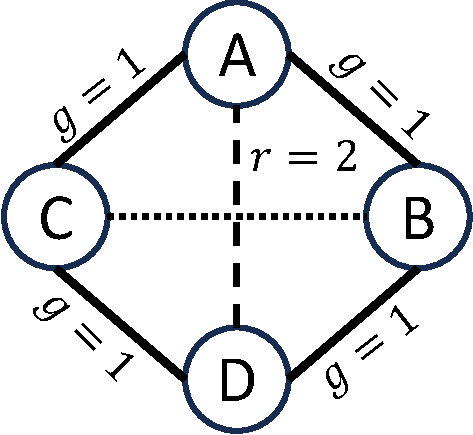
\includegraphics{Fig/BackPressure-MaxMin-CounterExample-crop.pdf}
\caption{A canonical example where the Max-min fair .}
\label{fig:maxmin-counterexample}
\end{figure}
\end{center}

Figure \ref{fig:maxmin-counterexample} depicts a small, 4-node network where Bell Pairs are generated at rate 1 along the solid corner edges between pairs (A,B), (A,C), (B,D) and (C,D), with consumption requests occurring only between (A,D) at rate 2.  The obvious optimal strategy is for both B and C to perform swaps that generate Bell pairs connecting A and D.

If we assume these generation events are stochastic in nature, such that small bursts upon a particular edge are not all that uncommon, note that the Max-min fair heuristic which does not explicitly consider consumption backlog would at times observe $Q_{BC} + 1 < \min(Q_{AB},Q_{AC}$ and/or 
$Q_{BC} + 1 < \min(Q_{CD},Q_{BD}$, in which cases the Bell pair $(B,C)$ would be created, consuming a Bell Pair on either AB and AC or on CD and BD.  Subsequently, were $Q_{BC}$ to grow sufficiently large, it could combine with one of the Bell Pairs along AB, AC, BD, BC to reconstitute only one Bell Pair, i.e., leading to a net loss in overall rate of generation of the needed AD pairs.  As such, a consumption rate of 2 could not be maintained. \Javad{can we include a simulation plot that actually shows the network is unstable (backlog for AD goes to infinity)? Do we have instability even when the consumption rate between C and B is $\epsilon>0$ for some small $\epsilon$? (This prevents naive schemes like not performing swap if direct pair does not have consumption rate) }

This phenomenon would be further exacerbated if there were multiple nodes of type B and C where the desired generation paths would be of the form $A-C_1-C_2-\ldots-C_n-D$ $A-B_1-B_2-\ldots-B_n-D$ such that every $Q_{B_iC_j}$ would need to be balanced.






\section{Dual LP}

We now form a \emph{Lagrangian} for the LP by dualizing the two families of inequalities \eqref{eq:Phard-balance} and \eqref{eq:Phard-demand}, but \emph{not} dualizing the node caps \eqref{eq:Phard-cap}.


We introduce dual variables:
\begin{itemize}[leftmargin=2em]
\item For each $xy$, let $\alpha_{xy}\ge 0$ be the Lagrange multiplier for the \emph{resource-balance} constraint \eqref{eq:Phard-balance}:
\[
r_{xy}
-
\Big(
g_{xy}
+\sum_{i\notin\{x,y\}}\sigma_i^{x,y}
-\sum_{w\notin\{x,y\}}(\sigma_x^{y,w}+\sigma_y^{x,w})
\Big)
\ \le\ 0.
\]

\item For each $xy$, let $\gamma_{xy}\ge 0$ be the Lagrange multiplier for the \emph{demand-satisfaction} constraint \eqref{eq:Phard-demand}:
\[
\lambda_{xy}-r_{xy} \ \le\ 0
\]
\end{itemize}

We can treat the LP feasibility as minimizing $0$ subject to the same constraints. Then the Lagrangian is
\begin{equation}
\begin{aligned}
\mathcal{L}(r,\sigma;\alpha,\gamma)
&:= \sum_{xy}\alpha_{xy}\,
\Big(
r_{xy}
-
g_{xy}
-\sum_{i\notin\{x,y\}}\sigma_i^{x,y}
+\sum_{w\notin\{x,y\}}(\sigma_x^{y,w}+\sigma_y^{x,w})
\Big) \\
&\quad
+ \sum_{xy}\gamma_{xy}\,(\lambda_{xy}-r_{xy}).
\end{aligned}
\label{eq:Lagrangian-expand}
\end{equation}
where $r, \sigma$ are subject to (\ref{eq:Phard-cap}) and (\ref{eq:sign}). Expanding and collecting $r$-terms and $\sigma$-terms, the Lagrangian is written as
\begin{equation}
\begin{aligned}
\mathcal{L}(r,\sigma;\alpha,\gamma)
&= \sum_{xy}(\alpha_{xy}-\gamma_{xy})\,r_{xy} \\
&\quad
+ \sum_i \sum_{y<y'} 
\Big(
\alpha_{iy}+\alpha_{iy'}
-\alpha_{yy'}
\Big)\,
\sigma_i^{y,y'} \\
&\quad
-\sum_{xy} \alpha_{xy}\,g_{xy}
+ \sum_{xy}\gamma_{xy}\,\lambda_{xy}.
\end{aligned}
\label{eq:Lagrangian-collected}
\end{equation}


For node $i$ and distinct $y,y'$, define
\begin{equation}
W_i(y,y')
:= \alpha_{yy'}-\alpha_{iy}-\alpha_{iy'}.
\label{eq:Wi-def}
\end{equation}
Then the $\sigma$-term in \eqref{eq:Lagrangian-collected} is:
\[
\sum_i \sum_{y<y'}
\sigma_i^{y,y'}\,
\big(
\alpha_{iy}+\alpha_{iy'}-\alpha_{yy'}
\big)
= \sum_i \sum_{y<y'} \sigma_i^{y,y'}\,\big(-W_i(y,y')\big).
\]
This shows that increasing $\sigma_i^{y,y'}$ is attractive if and only if $W_i(y,y')>0$. Thus $W_i(y,y')$ is exactly the \emph{marginal value} of using a swap at node $i$ to convert $[i,y]$ and $[i,y']$ into $[y,y']$.

\section{From dual to the online backpressure algorithm}

We now interpret \eqref{eq:Lagrangian-collected} as a per-slot objective. The idea is:
\begin{itemize}[leftmargin=2em]
\item At slot $t$, treat $(\gamma(t),\alpha(t))$ as current dual ``prices'',
\item Choose \emph{instantaneous} actions $(R(t),\mu(t))$ that maximize the per-slot Lagrangian subject to physical feasibility for that slot,
\item Then update $(\gamma,\alpha)$ via a projected subgradient step.
\end{itemize}

% \subsection{Per-slot decisions}

% In each slot $t$, the decisions are:
% \begin{itemize}[leftmargin=2em]

% \item $\mu_i^{y,y'}(t)$, how many swaps node $i$ performs across neighbors $y,y'$.

% \item $R_{xy}(t)$, how many $[x,y]$ we serve to satisfy demand.
% \end{itemize}

% The actions must satisfy the per-slot constraints:
% \begin{align}
% \sum_{\substack{y<y'\\ y,y'\neq i}}\mu_i^{y,y'}(t)
% &\le K_i,
% &&\forall i,t, \label{eq:slot-cap}\\
% \sum_{\substack{y'\neq y\\ y'\neq i}}\mu_i^{y,y'}(t)
% &\le Q_{iy}(t)+G_{iy}(t),
% &&\forall i,y\neq i,t, \label{eq:slot-avail}\\
% Q'_{xy}(t)
% &= Q_{xy}(t)+G_{xy}(t)
% + \sum_{i\notin\{x,y\}}\mu_i^{x,y}(t)
% - \sum_{w\notin\{x,y\}}\big(\mu_x^{y,w}(t)+\mu_y^{x,w}(t)\big),
% &&\forall xy,t,
% \label{eq:slot-Qprime}\\
% 0\ \le\ R_{xy}(t)
% &\le \min\{\,Q'_{xy}(t),\ D_{xy}(t)+A_{xy}(t), R_{\max}\,\},
% &&\forall xy,t,
% \label{eq:slot-Rbox}
% \end{align}
% and then evolve demand and inventory via \eqref{eq:D-backlog}, \eqref{eq:Q-evol}.

% Note that \eqref{eq:slot-cap} and \eqref{eq:slot-avail} are \emph{exactly} the instantaneous versions of the ``hard'' constraints in \eqref{eq:Phard-cap} and physical feasibility.

%\subsection{Instantaneous Lagrangian objective}

Using the Lagrangian \eqref{eq:Lagrangian-collected}, the slot-$t$ objective—ignoring constant terms that do not depend on $(R,\mu)$ in that slot—is
\begin{equation}
\begin{aligned}
\mathcal{L}_t(R,\mu;\alpha(t),\gamma(t))
&:= \sum_{xy}
\big(\gamma_{xy}(t)-\alpha_{xy}(t)\big)\,R_{xy}(t) \\
&\quad + \sum_i \sum_{y<y'}
\mu_i^{y,y'}(t)\,W_i(y,y';t),
\end{aligned}
\label{eq:inst-Lagrangian}
\end{equation}
where $W_i(y,y';t)$ is the weight \eqref{eq:Wi-def} evaluated at the current duals $\alpha(t)$.

In the \emph{online backpressure policy}, at each slot $t$, we choose $(R(t),\mu(t))$ to maximize \eqref{eq:inst-Lagrangian} subject to \eqref{eq:cap-phys}--\eqref{eq:Q-evol}.




\paragraph{Swap decision $\mu(t)$.}
For each node $i$, the contribution to \eqref{eq:inst-Lagrangian} is
\[
\sum_{\substack{y<y'\\ y,y'\neq i}}
\mu_i^{y,y'}(t)\,W_i(y,y';t).
\]
Node $i$ must respect its own physical caps/availability \eqref{eq:cap-phys}--\eqref{eq:avail-phys}. Thus node $i$ solves:
\begin{equation}
\begin{aligned}
\max_{\mu_i^{\cdot,\cdot}(t)\ge 0}\quad
&\sum_{\substack{y<y'\\ y,y'\neq i}}
\mu_i^{y,y'}(t)\,W_i(y,y';t) \\[2pt]
\text{s.t.}\quad
&\sum_{\substack{y<y'\\ y,y'\neq i}}
\mu_i^{y,y'}(t)\ \le\ K_i, \\
&\sum_{\substack{y'\neq y\\ y'\neq i}}
\mu_i^{y,y'}(t)
\ \le\ Q_{iy}(t)+G_{iy}(t),
\qquad \forall y\neq i.
\end{aligned}
\label{eq:nodeILP-detailed}
\end{equation}
The solution to the above optimization is as follows: Each node $i$ allocates up to $K_i$ swaps, subject to not over-consuming any $[i,y]$ link, to the
largest positive $W_i(y,y')$. If all $W_i(y,y')\le 0$, the optimum is $\mu_i^{y,y'}(t)=0$.

\paragraph{Service decision $R(t)$.}
Fix $xy$. Its contribution to \eqref{eq:inst-Lagrangian} is linear:
\[
(\gamma_{xy}(t)-\alpha_{xy}(t))\,R_{xy}(t).
\]
Subject to \eqref{eq:R-box}, the optimizer is:
\begin{equation}
R_{xy}(t)\;=\;
\begin{cases}
\min\!\big\{\,Q'_{xy}(t),\ D_{xy}(t)+A_{xy}(t)\,\big\},
&\text{if }\gamma_{xy}(t)\ge \alpha_{xy}(t),\\[4pt]
0, &\text{otherwise.}
\end{cases}
\label{eq:Rrule-detailed}
\end{equation}
This has the following interpretation:
\begin{itemize}[leftmargin=2em]
\item If $\gamma_{xy} \ge \alpha_{xy}$, unmet demand pressure outweighs scarcity pressure, so we serve as much as we physically can.
\item If $\gamma_{xy} < \alpha_{xy}$, resource scarcity is more ``valuable'' than clearing demand on this edge, so we hold back.
\end{itemize}


\section{Dual variable updates}\label{sec:primal-dual}

We now show how $\gamma(t)$ and $\alpha(t)$ evolve as projected subgradient ascent iterates on the dual problem. It is well known from primal-dual algorithms for classical network utility maximization, e.g., ~\cite{Stolyar2006GreedyPrimalDual, Neely2010StochasticNetworkOptimization}, that the evolution of the dual variables can be seen as queues whose dynamics provide a  stochastic approximation to the dual subgradient method. Specifically, the dual updates are as follows: 

The demand-satisfaction constraint \eqref{eq:Phard-demand} is $\lambda_{xy} - r_{xy} \le 0$.
In a single slot, we interpret $r_{xy}(t)=R_{xy}(t)$ and $\lambda_{xy}=A_{xy}(t)$. Then stochastic subgradient ascent on the dual, with unit step and projection onto $\mathbb{R}_+^{|\Pairs|}$, gives
% The \emph{violation} is
% \[
% h^{\rm dem}_{xy}(t) := A_{xy}(t)-R_{xy}(t).
% \]
\begin{align}
\gamma_{xy}(t{+}1)
=\Big[\,
\gamma_{xy}(t)+A_{xy}(t)-R_{xy}(t)
\,\Big]_+,
\label{eq:gamma-update-full}
\end{align}

The resource-balance constraint \eqref{eq:Phard-balance} is
\[
r_{xy} - 
\Big(
g_{xy}
+\sum_{i\notin\{x,y\}}\sigma_i^{x,y}
-\sum_{w\notin\{x,y\}}(\sigma_x^{y,w}+\sigma_y^{x,w})
\Big)
\ \le\ 0.
\]
Per slot we interpret $r_{xy}(t)=R_{xy}(t)$, $\sigma_i^{y,y'}(t)=\mu_i^{y,y'}(t)$, and $g_{xy}(t)=G_{xy}(t)$, then stochastic subgradient ascent on the dual (with
unit steps and projection onto $\mathbb{R}_+^{|\Pairs|}$) gives
% so the \emph{violation} is
% \begin{equation}
% \begin{aligned}
% h^{\rm res}_{xy}(t)
% &:= R_{xy}(t)
% -\Big(
% G_{xy}(t)
% +\sum_{i\notin\{x,y\}}\mu_i^{x,y}(t)
% -\sum_{w\notin\{x,y\}}\big(\mu_x^{y,w}(t)+\mu_y^{x,w}(t)\big)
% \Big)\\
% &= R_{xy}(t)
% + \sum_{w\notin\{x,y\}}\big(\mu_x^{y,w}(t)+\mu_y^{x,w}(t)\big)
% - \Big(
% G_{xy}(t)
% +\sum_{i\notin\{x,y\}}\mu_i^{x,y}(t)
% \Big).
% \end{aligned}
% \label{eq:hres-expand}
% \end{equation}


% Standard primal--dual control (a.k.a.\ stochastic subgradient ascent on the dual with
% unit steps and projection onto $\mathbb{R}_+^{|\Pairs|}$) gives:
\begin{align}
% \gamma_{xy}(t{+}1)
% &=\Big[\,
% \gamma_{xy}(t)+h^{\rm dem}_{xy}(t)
% \,\Big]_+
% =\Big[\,
% \gamma_{xy}(t)+A_{xy}(t)-R_{xy}(t)
% \,\Big]_+,
% \label{eq:gamma-update-full}\\[4pt]
\alpha_{xy}(t{+}1)
% &=\Big[\,
% \alpha_{xy}(t)+h^{\rm res}_{xy}(t)
% \,\Big]_+\nonumber\\
%&
=\Big[\,
\alpha_{xy}(t)
+ R_{xy}(t)
+ \sum_{w\notin\{x,y\}}\big(\mu_x^{y,w}(t)+\mu_y^{x,w}(t)\big)
- \Big(
G_{xy}(t)
+\sum_{i\notin\{x,y\}}\mu_i^{x,y}(t)
\Big)
\,\Big]_+.
\label{eq:alphares-update-full}
\end{align}

% \begin{remark} I can add more details on the derivations above, but the proof alternatively follows from the Lyapunov technique in the next section without knowing the projected subgradient stuff. 
% \end{remark}


The updates \eqref{eq:gamma-update-full} and \eqref{eq:alphares-update-full} are \emph{exactly} queue-like evolutions:
\begin{itemize}[leftmargin=2em]
\item $\gamma_{xy}(t)$ is essentially the demand backlog $D_{xy}(t)$ (compare \eqref{eq:gamma-update-full} to \eqref{eq:D-backlog}). Hence, $\gamma(t) \equiv D(t)$ 
\item $\alpha_{xy}(t)$ measures scarcity of $[x,y]$ pairs as inputs to swaps and service. It increases when we \emph{consume} $[x,y]$ via $R$ or via swaps at $x$ or $y$, and it decreases when we \emph{produce} $[x,y]$ via $G_{xy}$ or via swaps at third-party nodes.
\end{itemize}

%%%%%%%%%%%%%%%%%%%%%%%%%%%%%%%%%%%%%%%%%%%%%%%%%%%%%%%%%
%%%%%%%%%%%%%%%%%%%%%%%%%%%%%%%%%%%%%%%%%%%%%%%%%%

\section{Virtual backpressure and physical realization}
\label{sec:virtual-physical}

In this section, we introduce a \emph{virtual}
backpressure algorithm that operates purely at the LP level, without any truncation due to
Bell-pair availability, and a separate \emph{physical} realization algorithm that uses actual
Bell pairs to gradually fulfill the virtual swap and service decisions. This separation helps with the analysis as it removes the intertwine between the stochastic
primal--dual algorithm and the availability of Bell pairs.

\subsection{Virtual backpressure algorithm}

The virtual algorithm keeps track of dual queues $(\gamma_{xy}(t),\alpha_{xy}(t))$ as before,
but it no longer sees the physical inventory $Q_{xy}(t)$.
Instead, at each slot $t$ it chooses \emph{virtual} swap and service decisions
\[
\bigl(\tilde R_{xy}(t),\tilde\mu_i^{y,y'}(t)\bigr).
\]
At slot $t$, the virtual actions satisfy:
\begin{align}
0 \le \tilde R_{xy}(t) &\le {R}_{\max},
&& \forall xy, \label{eq:virt-R-cap}\\
\tilde\mu_i^{y,y'}(t) &\ge 0,
&& \forall i,y,y', \label{eq:virt-mu-nonneg}\\
\sum_{\substack{y<y'\\ y,y'\neq i}} \tilde\mu_i^{y,y'}(t)
&\le K_i, && \forall i. \label{eq:virt-node-cap}
\end{align}
As before, $R_{\max}$ and $K_i$ are fixed per-slot caps on service and swap. There is no constraint coupling $\tilde\mu$ or $\tilde R$ to the
physical $Q_{xy}(t)$.

\paragraph{Dual updates.}
Given virtual decisions $(\tilde R(t),\tilde\mu(t))$, the dual variables $(\gamma,\alpha)$ are updated exactly as before:
% . Specifically, define per-slot virtual residuals as:
% \begin{align}
% \tilde h^{\rm dem}_{xy}(t)
% &:= A_{xy}(t) - \tilde R_{xy}(t),
% \label{eq:virt-hdem}\\
% \tilde h^{\rm res}_{xy}(t)
% &:= \tilde R_{xy}(t)
% + \sum_{w\notin\{x,y\}} \bigl(\tilde\mu_x^{y,w}(t)+\tilde\mu_y^{x,w}(t)\bigr)
% - G_{xy}(t)
% - \sum_{i\notin\{x,y\}}\tilde\mu_i^{x,y}(t).
% \label{eq:virt-hres}
% \end{align}
% The dual queues $(\gamma,\alpha)$ are updated as:
\begin{align}
\gamma_{xy}(t{+}1)
& = \bigl[\gamma_{xy}(t) + A_{xy}(t) - \tilde R_{xy}(t)\bigr]_+,
\label{eq:virt-gamma-update}\\[1mm]
\alpha_{xy}(t{+}1)
&= \bigl[\alpha_{xy}(t) + \tilde R_{xy}(t)
+ \sum_{w\notin\{x,y\}} \bigl(\tilde\mu_x^{y,w}(t)+\tilde\mu_y^{x,w}(t)\bigr)
- G_{xy}(t)
- \sum_{i\notin\{x,y\}}\tilde\mu_i^{x,y}(t)\bigr]_+.
\label{eq:virt-alpha-update}
\end{align}
Thus $\gamma_{xy}$ measures the virtual demand backlog and $\alpha_{xy}$ measures virtual
resource scarcity, but both evolve purely according to the virtual decisions and do not see
physical queues.

\paragraph{Control rule.}
Given $(\gamma(t),\alpha(t))$, the backpresuure algorithm chooses $(\tilde R(t),\tilde\mu(t))$ as follows:
% to maximize the per-slot Lagrangian
% \begin{equation}
% \begin{aligned}
% \mathcal{L}^{\rm virt}_t(\tilde R,\tilde\mu;\gamma(t),\alpha(t))
% &:=
% \sum_{xy} (\gamma_{xy}(t)-\alpha_{xy}(t))\,\tilde R_{xy}(t) \\
% &\quad
% + \sum_i \sum_{y<y'}
% \tilde\mu_i^{y,y'}(t)\,W_i(y,y';t),
% \end{aligned}
% \label{eq:virt-Lagrangian}
% \end{equation}
% subject to~\eqref{eq:virt-R-cap}--\eqref{eq:virt-node-cap}.
Let $W_i(y,y';t)$ be the same weight as in~\eqref{eq:Wi-def}, evaluated at the current
$\alpha(t)$, i.e.,
\[
W_i(y,y';t)
= \alpha_{yy'}(t) - \alpha_{iy}(t) - \alpha_{iy'}(t).
\]

% Given $(\gamma(t),\alpha(t))$, the virtual backpressure algorithm chooses $(\tilde R(t),\tilde\mu(t))$ to maximize
% \eqref{eq:virt-Lagrangian} over~\eqref{eq:virt-R-cap}--\eqref{eq:virt-node-cap}. Then it ppdates $(\gamma,\alpha)$ via~\eqref{eq:virt-gamma-update}--\eqref{eq:virt-alpha-update}.

\textit{Swap rule:} 
 Each node $i$ finds:
% \begin{equation}
% \begin{aligned}
% \max_{\mu_i^{\cdot,\cdot}(t)\ge 0}\quad
% &\sum_{\substack{y<y'\\ y,y'\neq i}}
% \mu_i^{y,y'}(t)\,W_i(y,y';t) \\[2pt]
% \text{s.t.}\quad
% &\sum_{\substack{y<y'\\ y,y'\neq i}}
% \mu_i^{y,y'}(t)\ \le\ K_i, 
% \end{aligned}
% \label{eq:nodeILP-detailed}
% \end{equation}
\begin{equation}
\max_{\substack{y<y'\\ y,y'\neq i}}
W_i(y,y';t)
\label{eq:nodeILP-detailed}
\end{equation}
%The solution to the above optimization is simple: 
Let $uv$ be the pair with the maximum weight. If $W_i(u,v;t)\geq 0$, then node $i$ allocates $K_i$ swaps to  $uv$, i.e., $\mu_i^{u,v}(t)=K_i$. Otherwise, 
if $W_i(u,v;t)<0$, no swap is done, i.e., $\mu_i^{u,v}(t)=0$. 

\textit{Service rule:} For each $xy$, 
\begin{equation}
\tilde{R}_{xy}(t)\;=\;
\begin{cases}
\min\!\big\{R_{\max}, \gamma_{xy}(t)+A_{xy}(t)\,\big\},
&\text{if }\gamma_{xy}(t)\ge \alpha_{xy}(t),\\[4pt]
0, &\text{otherwise.}
\end{cases}
\label{eq:Rrule-detailed}
\end{equation}

% This is exactly the stochastic primal--dual algorithm for the LP in
% Section~\ref{sec:primal-dual}, now viewed as a self-contained virtual control system.




% Then, as $T \to \infty$, the time-averaged virtual swaps and services $\bar r(T)$ and $\bar{\sigma}(T)$ converge to some LP feasible rates $(r^\star,\sigma^\star)$.

% \begin{align}
% \liminf_{T\to\infty} \bar r_{xy}(T) &\ge \lambda_{xy},
% && \forall xy,
% \label{eq:virt-rate-demand}\\
% \limsup_{T\to\infty}
% \Bigl(
% \bar r_{xy}(T)
% - g_{xy}
% - \sum_{i\notin\{x,y\}} \bar\sigma_i^{x,y}(T)
% + \sum_{w\notin\{x,y\}}
% (\bar\sigma_x^{y,w}(T)+\bar\sigma_y^{x,w}(T))
% \Bigr)
% &\le 0,
% && \forall xy,
% \label{eq:virt-rate-balance}
% \end{align}
% and
% \begin{equation}
% \limsup_{T\to\infty}
% \frac{1}{T}\sum_{t=0}^{T-1}
% \E\!\big[\gamma_{xy}^2(t)+\alpha_{xy}^2(t)\big]
% < \infty.
% \label{eq:virt-dual-stability}
% \end{equation}


\subsection{Physical Bell-pair realization}

We now reconnect the virtual controller to the physical Bell-pair system.
The physical inventory $Q_{xy}(t)$ evolves according to exogenous generation and
\emph{realized} swaps and services, which are constrained by availability.

To decouple the virtual control from availability, we introduce \emph{deficit counters}:
\begin{itemize}[leftmargin=2em]
\item $H^R_{xy}(t)$: outstanding \emph{service} requests to consume Bell pairs $[x,y]$.
\item $H^\mu_i{}^{y,y'}(t)$: outstanding \emph{swap} requests at node $i$ that wish to
convert $[i,y]$ and $[i,y']$ into $[y,y']$.
\end{itemize}

The coupling between virtual and physical layers is as follows. At each slot $t$, after virtual decisions $(\tilde R(t),\tilde\mu(t))$ have been chosen:
\begin{align}
H^R_{xy}(t{+}1)
&= H^R_{xy}(t) + \tilde R_{xy}(t) - S^R_{xy}(t),
\label{eq:HR-update}\\
H^\mu_i{}^{y,y'}(t{+}1)
&= H^\mu_i{}^{y,y'}(t) + \tilde\mu_i^{y,y'}(t) - S^\mu_i{}^{y,y'}(t),
\label{eq:Hmu-update}
\end{align}
where $S^R_{xy}(t)$ and $S^\mu_i{}^{y,y'}(t)$ denote the \emph{number of requests actually
satisfied} in slot $t$ by the physical system (see below).

Thus $(H^R,H^\mu)$ track the deficit in fulfilling  promised operations:
whenever the virtual controller chooses $\tilde R_{xy}$ or $\tilde\mu_i^{y,y'}$, we enqueue
that many service/swap requests, and the physical layer fulfills them as Bell pairs become available.

\paragraph{Physical fulfillment rule.}
The physical system sees, at the beginning of slot $t$:
\[
\bigl(Q_{xy}(t), H^R_{xy}(t), H^\mu_i{}^{y,y'}(t)\bigr).
\]
It then:

\begin{enumerate}[leftmargin=2em,label=(\roman*)]
\item Generates new Bell pairs $G_{xy}(t)$ as before.
\item Chooses realized swaps $S^\mu_i{}^{y,y'}(t)$, subject to both:
  \begin{align}
  0 \le S^\mu_i{}^{y,y'}(t) &\le H^\mu_i{}^{y,y'}(t),
  && \forall i,y,y', \label{eq:Smu-leq-Hmu}\\
  \sum_{\substack{y<y'\\ y,y'\neq i}} S^\mu_i{}^{y,y'}(t)
  &\le K_i,
  && \forall i,
  \label{eq:Smu-node-cap}\\
  \sum_{\substack{y'\neq y\\ y'\neq i}} S^\mu_i{}^{y,y'}(t)
  &\le Q_{iy}(t)+G_{iy}(t),
  && \forall i,y\neq i,
  \label{eq:Smu-avail}
  \end{align}
  i.e., we can only realize swap requests that are in $H^\mu$ and for which both input links
  have Bell pairs available. The exact order of input pairs where available Bell pairs are used to realize the swaps is irrelevant. For example, in a greedy manner, node $i$ uses the Bell pairs on the input links to realize swaps and it stops when no further swap can be realized. This generates a maximal solution to 
  % a solution to 
  (\ref{eq:Smu-leq-Hmu})--(\ref{eq:Smu-node-cap})--(\ref{eq:Smu-avail}).
   
\item Updates an \emph{intermediate} inventory
  $Q'_{xy}(t)$ via the realized swaps $S^\mu$ exactly as in~\eqref{eq:Qprime-phys} with
  $\mu$ replaced by $S^\mu$.
\item Chooses realized service $S^R_{xy}(t)$ subject to
  \begin{align}
  0 \le S^R_{xy}(t)
  &\le \min\{Q'_{xy}(t),\,H^R_{xy}(t)\},
  && \forall xy,
  \label{eq:SR-leq-HR}
  \end{align}
  and then updates the physical inventory by
  \[
  Q_{xy}(t{+}1) = Q'_{xy}(t) - S^R_{xy}(t).
  \]
\end{enumerate}

Intuitively: the virtual controller produces a stream of swap and service \emph{requests} at
LP-feasible rates $(\tilde R,\tilde\mu)$.
The physical layer executes these requests as actual swaps and Bell-pair consumptions
whenever the needed Bell pairs are present; otherwise, the requests wait in $(H^R,H^\mu)$
until sufficient Bell pairs arrive.

\subsection{Analysis of decomposed algorithm }

The separation above suggests the following two-step strategy for analyzing throughput:

\begin{enumerate}[leftmargin=2em,label=(\roman*)]
\item \textbf{Virtual LP-feasible control.}
We can show that if $\lambda\in\mathrm{int}(\Lambda^K)$, then under the virtual backpressure controller
\eqref{eq:virt-gamma-update}--\eqref{eq:virt-alpha-update}--\eqref{eq:virt-Lagrangian} the
time-averaged virtual swaps and services $(\tilde R,\tilde\mu)$ lie in the capacity region
$\Lambda^K$, and the dual queues $(\gamma,\alpha)$ are stable. Specifically, let
\[
\bar r_{xy}(T)
:= \frac{1}{T}\sum_{t=0}^{T-1} \E[\tilde R_{xy}(t)],
\qquad
\bar\sigma_i^{y,y'}(T)
:= \frac{1}{T}\sum_{t=0}^{T-1} \E[\tilde\mu_i^{y,y'}(t)].
\]
Under the same assumptions as in Theorem~\ref{thm:main}, and using standard
stochastic primal--dual Lyapunov arguments, one can show that if $\lambda\in\mathrm{int}(\Lambda^K)$, dual prices $(\gamma,\alpha)$ are strongly stable, i.e., 
\begin{equation}
\limsup_{T\to\infty}
\frac{1}{T}\sum_{t=0}^{T-1}
\E\!\big[\gamma_{xy}^2(t)+\alpha_{xy}^2(t)\big]
< \infty.
\label{eq:virt-dual-stability}
\end{equation}
From which, it follows that $(\bar r(T), \bar \sigma (T))$ are LP-feasible rates as $T \to \infty$. 

\item \textbf{Physical fulfillment of virtual requests.}
Given any virtual control whose net per-link consumption rates are LP-feasible with slack,
analyze the coupled request queues $(H^R,H^\mu)$ and physical inventories $Q$ under the
fulfillment rule~\eqref{eq:HR-update}--\eqref{eq:Hmu-update}--\eqref{eq:Smu-leq-Hmu}--\eqref{eq:Smu-avail}--\eqref{eq:SR-leq-HR}.
In particular, show that in any fluid limit, the outstanding requests $(H^R,H^\mu)$ do not
grow on the fluid time scale (their fluid limits are identically zero), and the realized
swaps and services $(S^R,S^\mu)$ coincide almost everywhere with the virtual ones
$(\tilde R,\tilde\mu)$.

\end{enumerate}

Under this decomposition, throughput optimality of the \emph{overall} architecture follows
from:
(i) the virtual controller producing LP-feasible rates $(\tilde R,\tilde\mu)$ whenever
$\lambda\in\mathrm{int}(\Lambda^K)$, and
(ii) the physical layer being able to fulfill almost all virtual requests using the actual
Bell-pair inflows.




\section{Stability via Lyapunov analysis}

We now prove that if the consumption rates $\lambda$ are strictly inside the capacity region $\Lambda^K$, then under the online backpressure policy described above, both $\gamma(t)$ and $\alpha(t)$ remain strongly stable, and the long-run service rate meets (and slightly exceeds) demand.

\textbf{Lyapunov function.} Define the quadratic Lyapunov function
\begin{equation}
L(\gamma,\alpha)
:= \frac12 \sum_{xy}
\Big(
\gamma_{xy}^2 + \alpha^2_{xy}
\Big).
\label{eq:Lyap-def}
\end{equation}
Let $S(t)$ denote the full system state at the beginning of slot $t$, including $(\gamma(t),\alpha(t),Q(t))$ and any other needed components.
Define the conditional drift
\begin{equation}
\Delta(t)
:= \E\!\left[
L(\gamma(t{+}1),\alpha(t{+}1))
-
L(\gamma(t),\alpha(t))
\ \big|\ S(t)
\right].
\label{eq:drift-def}
\end{equation}

We will show if $\lambda\in\mathrm{int}(\Lambda^K)$,  we will get a \emph{negative drift outside a bounded set on $\alpha$ and $\gamma$}. Then stability follows from Foster-Lyapunov Theorem~\cite{meyn2012markov}. 

\textbf{Bounding the one-step drift}. For each coordinate of \eqref{eq:gamma-update-full}:
\begin{equation}
\begin{aligned}
\gamma_{xy}(t{+}1)^2 - \gamma_{xy}(t)^2
&\le
\big(A_{xy}(t)-R_{xy}(t)\big)^2
+ 2\,\gamma_{xy}(t)\,\big(A_{xy}(t)-R_{xy}(t)\big).
\end{aligned}
\label{eq:gamma-square-step}
\end{equation}
And, for each coordinate of \eqref{eq:alphares-update-full}:
\begin{equation}
\begin{aligned}
\alpha_{xy}(t{+}1)^2
- \alpha_{xy}(t)^2
&\le
\Big(
R_{xy}(t)
+ \sum_{w\notin\{x,y\}}\big(\mu_x^{y,w}(t)+\mu_y^{x,w}(t)\big)
- G_{xy}(t) 
- \sum_{i\notin\{x,y\}}\mu_i^{x,y}(t)
\Big)^2 \\
&\quad
+ 2\,\alpha_{xy}(t)\Big[
R_{xy}(t)
+ \sum_{w\notin\{x,y\}}\big(\mu_x^{y,w}(t)+\mu_y^{x,w}(t)\big)
- G_{xy}(t) \\
&\qquad
- \sum_{i\notin\{x,y\}}\mu_i^{x,y}(t)
\Big].
\end{aligned}
\label{eq:alphares-square-step}
\end{equation}










We sum \eqref{eq:gamma-square-step} and \eqref{eq:alphares-square-step} over all $xy$, divide by $2$, and then take conditional expectation given $S(t)$.
Because $A_{xy}(t)$ and $G_{xy}(t)$ have bounded second moments, $R_{xy}(t)$ and $\mu_i^{y,y'}(t)$ are bounded by the hard caps  \eqref{eq:R-box} and \eqref{eq:cap-phys}, \emph{all} the quadratic terms can be absorbed into a constant $B<\infty$ that depends only on $R_{\max}, \{K_i\}$, and the second moments of $\{G_{xy}(t)\}$ and $\{A_{xy}(t)\}$.  We obtain:
\begin{equation}
\begin{aligned}
\Delta(t)\ \le\ &
B\\
&+ \sum_{xy} \gamma_{xy}(t)\,
\E\!\left[ A_{xy}(t)-R_{xy}(t)\ \big|\ S(t)\right] \\
&+ \sum_{xy} \alpha_{xy}(t)\,
\E\!\Big[
R_{xy}(t)
+ \sum_{w\notin\{x,y\}}\big(\mu_x^{y,w}(t)+\mu_y^{x,w}(t)\big) \\
&\qquad\qquad\qquad
- G_{xy}(t)
- \sum_{i\notin\{x,y\}}\mu_i^{x,y}(t)
\ \Big|\ S(t)\Big].
\end{aligned}
\label{eq:drift-before-rearrange}
\end{equation}

Now use $\E[A_{xy}(t)]=\lambda_{xy}$ and $\E[G_{xy}(t)]=g_{xy}$:
\begin{equation}
\begin{aligned}
\Delta(t)\ \le\ &
B
+ \sum_{xy} \gamma_{xy}(t)\,
\big(\lambda_{xy} - \E[R_{xy}(t)\mid S(t)]\big) \\
&+ \sum_{xy} \alpha_{xy}(t)\,
\E\!\Big[
R_{xy}(t)
+ \sum_{w\notin\{x,y\}}\big(\mu_x^{y,w}(t)+\mu_y^{x,w}(t)\big)
- \sum_{i\notin\{x,y\}}\mu_i^{x,y}(t)
\ \Big|\ S(t)\Big]\\
&- \sum_{xy} \alpha_{xy}(t)\,g_{xy},
\end{aligned}
\label{eq:drift-rearrange}
\end{equation} Note
\[
\sum_{xy} \alpha_{xy}(t)
\Big(
\sum_{w\notin\{x,y\}}\big(\mu_x^{y,w}(t)+\mu_y^{x,w}(t)\big)
- \sum_{i\notin\{x,y\}}\mu_i^{x,y}(t)
\Big)
= - \sum_i \sum_{y<y'}
\mu_i^{y,y'}(t)\,W_i(y,y';t),
\]
where $W_i$ is from \eqref{eq:Wi-def}. 
% This identity is standard: Intuitively, each swap $\mu_i^{y,y'}$ \emph{consumes} entanglement on the input links $[i,y]$ and $[i,y']$ and \emph{creates} entanglement on the output link $[y,y']$. Thus, the scarcity prices $\alpha_{iy},\alpha_{iy'}$ increase while $\alpha_{yy'}$ decrease, and the net contribution of this swap to the Lagrangian is exactly $-\mu_i^{y,y'} W_i(y,y')$.
Plugging in \eqref{eq:drift-rearrange}, we get
\begin{equation}
\begin{aligned}
\Delta(t)\ \le\ &
B
+ \sum_{xy} \gamma_{xy}(t)\,
\big(\lambda_{xy} - \E[R_{xy}(t)\mid S(t)]\big) \\
&+ \sum_{xy} \alpha_{xy}(t)\,
\E[R_{xy}(t)\mid S(t)]
- \sum_i \E\!\Big[\sum_{y<y'}\mu_i^{y,y'}(t)\,W_i(y,y';t)\ \Big|\ S(t)\Big] \\
&- \sum_{xy} \alpha_{xy}(t)\,g_{xy}.
\end{aligned}
\label{eq:drift-node-form}
\end{equation}

Now specialize to the backpressure policy and compare its one-step decisions with those of an arbitrary alternative feasible policy $\tilde{\pi}$. By construction,
our backpressure policy $(R(t),\mu(t))$ \emph{maximizes} the instantaneous Lagrangian \eqref{eq:inst-Lagrangian} over the physical constraints at slot $t$. Therefore:
\begin{align}
\sum_{xy} (\gamma_{xy}(t)-\alpha_{xy}(t))
\E\!\left[R_{xy}(t)\mid\cdot\right]
&\ge
\sum_{xy} (\gamma_{xy}(t)-\alpha_{xy}(t))
\E\!\left[R_{xy}^{\tilde\pi}(t)\mid\cdot\right],
\label{eq:maxweight-service}\\
\sum_i \E\!\left[\sum_{y<y'} \mu_i^{y,y'}(t)\,W_i(y,y';t)\mid\cdot\right]
&\ge
\sum_i \E\!\left[\sum_{y<y'} (\mu_i^{y,y'})^{\tilde\pi}(t)\,W_i(y,y';t)\mid\cdot\right].
\label{eq:maxweight-swap}
\end{align}

% We rewrite \eqref{eq:drift-node-form} using \eqref{eq:maxweight-service}--\eqref{eq:maxweight-swap} with $\tilde\pi := \pi^\star$, a particular stationary randomized policy described below.

% \textbf{Slack policy under interior load.} 
% If $\lambda\in\mathrm{int}(\Lambda^K)$, then there exists $\epsilon>0$ and a feasible $(r,\sigma)$ for the LP such that
% \[
% r_{xy} \ge \lambda_{xy}+\epsilon
% \quad\text{and}\quad
% r_{xy} \le g_{xy}
% +\sum_{i\notin\{x,y\}}\sigma_i^{x,y}
% -\sum_{w\notin\{x,y\}}(\sigma_x^{y,w}+\sigma_y^{x,w}),
% \]
% and $\sum_{y<y'}\sigma_i^{y,y'}\le K_i$.
% By standard time-sharing arguments, we can build a \emph{stationary randomized per-slot policy} $\pi^\star$ that achieves per-slot expectations
% \[
% \E_{\pi^\star}[R_{xy}(t)] = r_{xy},\qquad
% \E_{\pi^\star}[\mu_i^{y,y'}(t)] = \sigma_i^{y,y'},
% \]
% while obeying \eqref{eq:slot-cap}--\eqref{eq:slot-Rbox} almost surely.

% Under $\pi^\star$ we therefore have
% \begin{align}
% \E_{\pi^\star}[R_{xy}(t)] &\ge \lambda_{xy}+\epsilon, \label{eq:piR-ineq}\\
% \E_{\pi^\star}\!\left[
% R_{xy}(t)
% + \sum_{w\notin\{x,y\}}\big(\mu_x^{y,w}(t)+\mu_y^{x,w}(t)\big)
% - \sum_{i\notin\{x,y\}}\mu_i^{x,y}(t)
% \right]
% &\le
% g_{xy}, \label{eq:pi-balance-ineq}
% \end{align}
% for all $xy$.

% \textbf{Final drift inequality.} 
% Plug $\tilde\pi=\pi^\star$ into \eqref{eq:maxweight-service}--\eqref{eq:maxweight-swap}, then substitute into \eqref{eq:drift-node-form}:

% \begin{equation}
% \begin{aligned}
% \Delta(t)
% &\le B
% + \sum_{xy} \gamma_{xy}(t)\,
% \big(\lambda_{xy} - \E_{\pi^\star}[R_{xy}(t)]\big)
% \\
% &\quad
% + \sum_{xy} \alpha_{xy}(t)\,
% \Big(
% \E_{\pi^\star}[R_{xy}(t)]
% - g_{xy}
% + \E_{\pi^\star}\!\big[
% \sum_{w\notin\{x,y\}}(\mu_x^{y,w}(t)+\mu_y^{x,w}(t))
% - \sum_{i\notin\{x,y\}}\mu_i^{x,y}(t)
% \big]
% \Big).
% \end{aligned}
% \label{eq:drift-pre-simplify}
% \end{equation}

% Now apply \eqref{eq:piR-ineq} and \eqref{eq:pi-balance-ineq}:
% \begin{align*}
% \lambda_{xy} - \E_{\pi^\star}[R_{xy}(t)]
% &\le -\epsilon,\\
% \E_{\pi^\star}[R_{xy}(t)]
% - g_{xy}
% + \E_{\pi^\star}\!\big[
% \sum_{w}(\mu_x^{y,w}+\mu_y^{x,w})
% - \sum_{i}\mu_i^{x,y}
% \big]
% &\le 0.
% \end{align*}
% Therefore
% \begin{equation}
% \Delta(t)
% \ \le\
% B
% -\epsilon\,\sum_{xy}\gamma_{xy}(t).
% \label{eq:final-drift}
% \end{equation}

% \textbf{Stability and throughput optimality.} Inequality \eqref{eq:final-drift} says: outside a bounded set (where $\sum\gamma_{xy}$ is large), the expected Lyapunov drift is strictly negative. By a standard Foster--Lyapunov argument for Markov chains with countable state (or the stochastic network stability framework), this implies \emph{strong stability} of $\gamma(t)$, i.e.,
% \[
% \limsup_{T\to\infty}\frac{1}{T}\sum_{t=0}^{T-1}\sum_{xy}\E[\gamma_{xy}(t)]
% \ <\ \infty.
% \]
% Because $\alpha(t)$ is also in the Lyapunov function \eqref{eq:Lyap-def} and its contribution to $\Delta(t)$ is nonpositive in \eqref{eq:final-drift}, we similarly get strong stability of $\alpha(t)$.

% Finally, rearranging the queue update \eqref{eq:gamma-update-full} in steady state and summing over $t$ gives
% \[
% \frac{1}{T}\sum_{t=0}^{T-1}\E[R_{xy}(t)]
% \ \ge\
% \lambda_{xy}
% - \frac{\E[\gamma_{xy}(T)]-\E[\gamma_{xy}(0)]}{T}.
% \]
% Taking $T\to\infty$ and using stability of $\gamma$ shows
% \[
% \liminf_{T\to\infty}
% \frac{1}{T}\sum_{t=0}^{T-1}\E[R_{xy}(t)]
% \ \ge\ \lambda_{xy},
% \qquad \forall xy.
% \]
% i.e., the average service rate is at least the consumption rate.

We rewrite \eqref{eq:drift-node-form} using \eqref{eq:maxweight-service}--\eqref{eq:maxweight-swap} with $\tilde\pi$:

% \textbf{Slack policy under interior load.} 
% If $\lambda\in\mathrm{int}(\Lambda^K)$, then there exists $\epsilon>0$ and a feasible $(r,\sigma)$ for the LP such that
% \[
% r_{xy} \ge \lambda_{xy}+\epsilon
% \quad\text{and}\quad
% r_{xy} \le g_{xy}
% +\sum_{i\notin\{x,y\}}\sigma_i^{x,y}
% -\sum_{w\notin\{x,y\}}(\sigma_x^{y,w}+\sigma_y^{x,w}),
% \]
% and $\sum_{y<y'}\sigma_i^{y,y'}\le K_i$.
% By standard time-sharing arguments, we can build a \emph{stationary randomized per-slot policy} $\pi^\star$ that achieves per-slot expectations
% \[
% \E_{\pi^\star}[R_{xy}(t)] = r_{xy},\qquad
% \E_{\pi^\star}[\mu_i^{y,y'}(t)] = \sigma_i^{y,y'},
% \]
% while obeying \eqref{eq:slot-cap}--\eqref{eq:slot-Rbox} almost surely.

% Under $\pi^\star$ we therefore have
% \begin{align}
% \E_{\pi^\star}[R_{xy}(t)] &\ge \lambda_{xy}+\epsilon, \label{eq:piR-ineq}\\
% \E_{\pi^\star}\!\left[
% R_{xy}(t)
% + \sum_{w\notin\{x,y\}}\big(\mu_x^{y,w}(t)+\mu_y^{x,w}(t)\big)
% - \sum_{i\notin\{x,y\}}\mu_i^{x,y}(t)
% \right]
% &\le
% g_{xy}, \label{eq:pi-balance-ineq}
% \end{align}
% for all $xy$.

% \textbf{Final drift inequality.} 
% Plug $\tilde\pi=\pi^\star$ into \eqref{eq:maxweight-service}--\eqref{eq:maxweight-swap}, then substitute into \eqref{eq:drift-node-form}:

\begin{equation}
\begin{aligned}
\Delta(t)
&\le B
+ \sum_{xy} \gamma_{xy}(t)\,
\big(\lambda_{xy} - \E_{\tilde\pi}[R_{xy}(t)\mid S(t)]\big)
\\
&\quad
+ \sum_{xy} \alpha_{xy}(t)\,
\Big(
\E_{\tilde\pi}\big[R_{xy}(t) + H_{xy}(t)  \mid S(t)
\big] - g_{xy}
\Big),
\end{aligned}
\label{eq:drift-pre-simplify}
\end{equation}
where 
\begin{equation}
H_{xy}(t) = \sum_{w\notin\{x,y\}}(\mu_x^{y,w}(t)+\mu_y^{x,w}(t))
- \sum_{i\notin\{x,y\}}\mu_i^{x,y}(t) 
\label{eq:H}
\end{equation}
and $\E_{\tilde\pi}[\cdot\mid S(t)]$ denotes expectation when,
starting from state $S(t)$ at time $t$, the system is controlled
by $\tilde \pi$.
\subsection{Comparison policy and frame-average inequalities} \label{sec:comparison}

Assume $\lambda\in\mathrm{int}(\Lambda^K)$.  As in the LP argument,
there exist $\epsilon>0$ and a feasible point $(r,\sigma)$ for the LP
such that
\[
r_{xy} \ge \lambda_{xy}+\epsilon,\qquad
r_{xy} +\sum_{i\notin\{x,y\}}\sigma_i^{x,y}
-\sum_{w\notin\{x,y\}}(\sigma_x^{y,w}+\sigma_y^{x,w}) \le g_{xy}
,
\]
and $\sum_{y<y'}\sigma_i^{y,y'}\le K_i$ for all $i$.

We now assume that there exists a (possibly queue-aware) Markov policy $\pi^\star$ that implements these LP flows in the
following sense: there is a constant $C<\infty$ and a (possibly
state-dependent) frame length $\eta :=\eta(S(t)) \in\mathbb{Z}_{\ge 1}$ such that
given initial state $S(t)$ and all unordered pairs $xy$,
\begin{align}
\frac{1}{\eta}\,
\E_{\pi^\star}\!\left[
\sum_{\tau=t}^{t+\eta-1}
R_{xy}(\tau)
\ \Big|\ S(t)
\right]
&\ge
\lambda_{xy}+\epsilon
-\frac{C}{\eta},
\qquad \forall xy,
\label{eq:pistar-frame-demand-avg-again}\\[1mm]
\frac{1}{\eta}\,
\E_{\pi^\star}\!\left[
\sum_{\tau=t}^{t+\eta-1}
R_{xy}(\tau)+H_{xy}(\tau)
\ \Big|\ S(t)
\right]
&\le g_{xy}+\frac{C}{\eta},
\qquad \forall xy.
\label{eq:pistar-frame-res-avg-again}
\end{align}
These are simply fluid-limit interpretations of the LP, and they express the fact that, over a sufficiently long window of time $\eta$, we can serve the demand at a rate at least
$\lambda_{xy}+\epsilon$, up to a vanishing $O(1/\eta)$ error, and 
satisfy the resource-balance constraint, again up to vanishing $O(1/\eta)$. 
%Such a policy can be constructed, for example, by tracking the LP
%target flows $(r,\sigma)$ with additional ``deficit counters'' and
%applying a longest-deficit-first rule at each node; 
The existence of
$\pi^\star$ with
\eqref{eq:pistar-frame-demand-avg-again}--\eqref{eq:pistar-frame-res-avg-again}
is a fluid-limit consequence of LP feasibility and interiority, but we do not attempt to prove it here and take it as a comparison policy.

\textbf{Stability and throughput optimality.} 
We now compare the multi-slot drift of backpressure to the
performance of the comparison policy $\pi^\star$ from
Section~\ref{sec:comparison}.

%\subsection{Multi-slot drift as sum of one-step drifts}

Given an integer $\eta\ge 1$, define the $\eta$-slot drift
starting at time $t$ by
\begin{equation}
\Delta_\eta(t)
:=
\E\!\left[
L(\gamma(t{+}\eta),\alpha(t{+}\eta))
-
L(\gamma(t),\alpha(t))
\ \Big|\ S(t)
\right].
\label{eq:Delta-eta-def}
\end{equation}

\begin{lemma}[Multi-slot drift]
\label{lem:multi-slot}
For any $\eta\ge 1$ and any $t$,
\begin{equation}
\Delta_\eta(t)
=
\sum_{\tau=t}^{t+\eta-1}
\E\!\left[
\Delta(\tau)\ \Big|\ S(t)
\right].
\label{eq:multi-slot-sum}
\end{equation}
\end{lemma}

\begin{proof}
By telescoping,
\[
L(\gamma(t{+}\eta),\alpha(t{+}\eta))
-
L(\gamma(t),\alpha(t))
=
\sum_{\tau=t}^{t+\eta-1}
\Big(
L(\gamma(\tau{+}1),\alpha(\tau{+}1))
-
L(\gamma(\tau),\alpha(\tau))
\Big).
\]
Taking conditional expectation given $S(t)$ yields
\[
\Delta_\eta(t)
=
\sum_{\tau=t}^{t+\eta-1}
\E\!\left[
L(\gamma(\tau{+}1),\alpha(\tau{+}1))
-
L(\gamma(\tau),\alpha(\tau))
\ \Big|\ S(t)
\right].
\]
For each $\tau$, apply the tower property of condidional expectation, and use the definition of $\Delta(\tau)$ by
\eqref{eq:drift-def},
% \[
% \E\!\left[
% L(\gamma(\tau{+}1),\alpha(\tau{+}1))
% -
% L(\gamma(\tau),\alpha(\tau))
% \ \Big|\ X(t)
% \right]
% =
% \E\!\left[
% \E\big[
% L(\gamma(\tau{+}1),\alpha(\tau{+}1))
% -
% L(\gamma(\tau),\alpha(\tau))
% \ \big|\ X(\tau)
% \big]
% \ \Big|\ X(t)
% \right].
% \]
% The inner conditional expectation is exactly $\Delta(\tau)$ by
% \eqref{eq:Delta-one-step-def}, hence
% \[
% \E\!\left[
% L(\gamma(\tau{+}1),\alpha(\tau{+}1))
% -
% L(\gamma(\tau),\alpha(\tau))
% \ \Big|\ X(t)
% \right]
% =
% \E\!\left[
% \Delta(\tau)\ \Big|\ X(t)
% \right].
% \]
then substituting back yields \eqref{eq:multi-slot-sum}.
\end{proof}

Lemma~\ref{lem:multi-slot} shows that the $\eta$-slot drift is
exactly the sum, over the window $[t,t{+}\eta)$, of the expected
one-step drifts, all conditioned on the initial state $S(t)$.



Applying the comparison bound
\eqref{eq:drift-pre-simplify} at each $\tau$ and then using the
tower property again, we obtain
\begin{equation}
\begin{aligned}
\Delta_{\eta}(t)
&\le
B\,\eta
+ \sum_{\tau=t}^{t+\eta-1}
\sum_{xy} \E_{\pi^{\rm BP}}\!\Big[
\gamma_{xy}(\tau)\big(\lambda_{xy}
- \E_{\pi^\star}[R_{xy}(\tau)\mid S(\tau)]\big)
\;\Big|\; S(t)
\Big]\\
&\qquad
+ \sum_{\tau=t}^{t+\eta-1}
\sum_{xy} \E_{\pi^{\rm BP}}\!\Big[
\alpha_{xy}(\tau) \big(
\E_{\pi^\star}[R_{xy}(\tau)+H_{xy}(\tau)\mid S(\tau)] -g_{xy}
\big)\Big|\; S(t)
\Big].
\end{aligned}
\label{eq:frame-drift-preavg}
\end{equation}

At this point we use that the dual queues are nonnegative,
$\gamma_{xy}(\tau)\ge 0$ and $\alpha_{xy}(\tau)\ge 0$, and we combine
this with the \emph{frame-average} properties of $\pi^\star$ in
\eqref{eq:pistar-frame-demand-avg-again}--\eqref{eq:pistar-frame-res-avg-again}.
For any fixed $xy$ and state $S(t)$, write
\[
\overline{R}_{xy}^{\pi^\star}(t)
:=
\frac{1}{\eta}
\E_{\pi^\star}\!\left[
\sum_{\tau=t}^{t+\eta-1}
R_{xy}(\tau)
\;\Big|\; S(t)
\right],
\qquad
\overline{h}^{\rm res}_{xy,\pi^\star}(t)
:=
\frac{1}{\eta}
\E_{\pi^\star}\!\left[
\sum_{\tau=t}^{t+\eta-1}
h^{\rm res}_{xy}(\tau)
\;\Big|\; S(t)
\right].
\]
Then by \eqref{eq:pistar-frame-demand-avg-again} and
\eqref{eq:pistar-frame-res-avg-again},
\begin{align}
\overline{R}_{xy}^{\pi^\star}(t)
&\ge \lambda_{xy}+\epsilon - C/\eta_t,
\label{eq:Rbar-lower}\\
\overline{h}^{\rm res}_{xy,\pi^\star}(t)
&\le -\epsilon + C/\eta_t.
\label{eq:hbar-upper}
\end{align}

Using linearity of expectation and the nonnegativity of $\gamma$ and
$\alpha$, we can bound the sum in
\eqref{eq:frame-drift-preavg} as
\begin{equation}
\begin{aligned}
\Delta_{\pi^{\rm BP}}^{(\eta)}(t)
&\le
B\,\eta_t
+ \sum_{xy}
\E_{\pi^{\rm BP}}\!\left[
\sum_{\tau=t}^{t+\eta_t-1}
\gamma_{xy}(\tau)
\;\Big|\; X(t)
\right]\,
\big(\lambda_{xy} - \overline{R}_{xy}^{\pi^\star}(t)\big)\\
&\qquad
+ \sum_{xy}
\E_{\pi^{\rm BP}}\!\left[
\sum_{\tau=t}^{t+\eta_t-1}
\alpha_{xy}(\tau)
\;\Big|\; X(t)
\right]\,
\overline{h}^{\rm res}_{xy,\pi^\star}(t).
\end{aligned}
\label{eq:frame-drift-using-averages}
\end{equation}

Substituting \eqref{eq:Rbar-lower}--\eqref{eq:hbar-upper} and rearranging,
there exist constants $c_1,c_2>0$ and $B'<\infty$ such that, for
$\eta_t$ large enough,
\begin{equation}
\Delta_{\pi^{\rm BP}}^{(\eta)}(t)
\ \le\
B'
- c_1
\sum_{xy}
\E_{\pi^{\rm BP}}\!\left[
\sum_{\tau=t}^{t+\eta_t-1}\gamma_{xy}(\tau)
\;\Big|\; X(t)
\right]
- c_2
\sum_{xy}
\E_{\pi^{\rm BP}}\!\left[
\sum_{\tau=t}^{t+\eta_t-1}\alpha_{xy}(\tau)
\;\Big|\; X(t)
\right].
\label{eq:frame-drift-negative}
\end{equation}

Intuitively, when the dual queues are large, the frame drift is
\emph{strictly negative} in the sense of
\eqref{eq:frame-drift-negative}: over each frame the Lyapunov
function $L$ is pulled downwards by an amount proportional to the
cumulative dual backlog within that frame.

\subsection{Application of random-time drift theorem}

Consider the embedded chain sampled at the random frame-start times
$\{t_k\}_{k\ge 0}$ defined by $t_0=0$ and
$t_{k+1}=t_k+\eta_{t_k}$.  Define
\[
\Phi_k := X(t_k),\qquad
V(\Phi_k) := L(\gamma(t_k),\alpha(t_k)).
\]
Then \eqref{eq:frame-drift-negative} is a random-time drift condition
of the general form studied in \cite{YukselMeyn2013}: there exist
constants $b<\infty$ and $\delta>0$ such that, outside a suitably
large compact set,
\begin{equation}
\E\!\left[
V(\Phi_{k+1})-V(\Phi_k)\;\big|\;\Phi_k
\right]
\ \le\
-b.
\label{eq:random-time-drift-condition}
\end{equation}
Moreover, the frame lengths $\eta_{t_k}$ are almost surely finite and
have finite first moment.

By the random-time, state-dependent drift theorem for Markov chains
(Y\"uksel--Meyn \cite[Theorem~2.1]{YukselMeyn2013}), the drift
condition \eqref{eq:random-time-drift-condition} implies that the
embedded chain $\{\Phi_k\}$ is positive Harris recurrent and that the
Lyapunov function $V(\Phi_k)$ has finite steady-state mean.  Because
$L$ controls $\sum_{xy}\gamma_{xy}^2$ and
$\sum_{xy}\alpha_{xy}^2$, this in turn implies strong stability of the
dual queues:
\[
\limsup_{T\to\infty}
\frac{1}{T}\sum_{t=0}^{T-1}
\sum_{xy}\E[\gamma_{xy}(t)] < \infty,
\qquad
\limsup_{T\to\infty}
\frac{1}{T}\sum_{t=0}^{T-1}
\sum_{xy}\E[\alpha_{xy}(t)] < \infty.
\]

Finally, as in the one-step proof, the demand-queue recursion
\eqref{eq:gamma-update-full} combined with the stability of $\gamma$
gives
\[
\liminf_{T\to\infty}
\frac{1}{T}\sum_{t=0}^{T-1}
\E[R_{xy}(t)]
\ \ge\
\lambda_{xy},
\qquad \forall xy\in\Pairs.
\]
We conclude that the backpressure policy $\pi^{\rm BP}$ is
throughput-optimal whenever $\lambda\in\mathrm{int}(\Lambda^K)$.







Inequality \eqref{eq:final-drift} says: outside a bounded set (where $\sum\gamma_{xy}$ is large), the expected Lyapunov drift is strictly negative. By a standard Foster--Lyapunov argument for Markov chains with countable state (or the stochastic network stability framework), this implies \emph{strong stability} of $\gamma(t)$, i.e.,
\[
\limsup_{T\to\infty}\frac{1}{T}\sum_{t=0}^{T-1}\sum_{xy}\E[\gamma_{xy}(t)]
\ <\ \infty.
\]
Because $\alpha(t)$ is also in the Lyapunov function \eqref{eq:Lyap-def} and its contribution to $\Delta(t)$ is nonpositive in \eqref{eq:final-drift}, we similarly get strong stability of $\alpha(t)$.

Finally, rearranging the queue update \eqref{eq:gamma-update-full} in steady state and summing over $t$ gives
\[
\frac{1}{T}\sum_{t=0}^{T-1}\E[R_{xy}(t)]
\ \ge\
\lambda_{xy}
- \frac{\E[\gamma_{xy}(T)]-\E[\gamma_{xy}(0)]}{T}.
\]
Taking $T\to\infty$ and using stability of $\gamma$ shows
\[
\liminf_{T\to\infty}
\frac{1}{T}\sum_{t=0}^{T-1}\E[R_{xy}(t)]
\ \ge\ \lambda_{xy},
\qquad \forall xy.
\]
i.e., the average service rate is at least the consumption rate.

We summarize this as our main result.

\begin{theorem}[Throughput optimality of Backpressure]
\label{thm:main}
Suppose $\lambda\in\mathrm{int}(\Lambda^K)$. Consider the following distributed policy:

\begin{enumerate}[leftmargin=2em,label=(\roman*)]
\item \textbf{At each slot $t$:} compute the weights
\[
W_i(y,y';t)=\alpha_{yy'}(t)-\alpha_{iy}(t)-\alpha_{iy'}(t).
\]

\item \textbf{Swaps at node $i$:} choose $\mu_i^{y,y'}(t)$ to solve the local max-weight \eqref{eq:nodeILP-detailed} subject to the instantaneous hard cap \eqref{eq:cap-phys} and availability constraints \eqref{eq:avail-phys}.

\item \textbf{Service on pair $xy$:} choose $R_{xy}(t)$ according to \eqref{eq:Rrule-detailed} (or equivalently, serve the full box upper bound whenever desired).

\item \textbf{Update dual queues:}
\begin{align*}
\gamma_{xy}(t{+}1)
&=\big[\gamma_{xy}(t)+A_{xy}(t)-R_{xy}(t)\big]_+,\\
\alpha_{xy}(t{+}1)
&=\Big[\alpha_{xy}(t)
+ R_{xy}(t)
+ \sum_{w\notin\{x,y\}}\big(\mu_x^{y,w}(t)+\mu_y^{x,w}(t)\big)\\
&\qquad\qquad
- \Big(G_{xy}(t)+\sum_{i\notin\{x,y\}}\mu_i^{x,y}(t)\Big)
\Big]_+.
\end{align*}
\end{enumerate}

Then both queues $\gamma(t)$ and $\alpha(t)$ are strongly stable, and the long-run average service rate meets the demand rate:
\[
\liminf_{T\to\infty}
\frac1T \sum_{t=0}^{T-1}\E[R_{xy}(t)]
\ \ge\ \lambda_{xy},
\quad \forall xy\in\Pairs.
\]
\end{theorem}

\section*{Discussion}

\begin{remark}[Why two queues are necessary]
The queue $\gamma_{xy}(t)$ acts like an ordinary demand backlog: it grows when arrivals $A_{xy}(t)$ exceed service $R_{xy}(t)$. The queue $\alpha_{xy}(t)$ is \emph{not} physical backlog but a scarcity shadow price: it grows when link $[x,y]$ is ``over-used'' as an input to swaps or for service, compared to how much it is replenished by generation or swaps \emph{into} $[x,y]$. The combination enforces both ``serve requests'' and ``don't overconsume scarce entanglement''.
\end{remark}

\begin{remark}[Decentralization]
Node $i$ needs:
\begin{itemize}[leftmargin=2em]
\item $\alpha_{iy}(t)$ for every neighbor $y$ to price consuming $[i,y]$ as a swap input,
\item $\alpha_{yy'}(t)$ for $(y,y')$ pairs it can create.
\end{itemize}
This information can be exchanged locally (gossip). Each node then solves \eqref{eq:nodeILP-detailed} independently.
\end{remark}

\section{Extension to Distillation Operation}
\label{sec:distillation-extension}

So far, we assumed that each logical operation
(serving one consumption request or performing one entanglement swap)
consumes exactly \emph{one} Bell pair on each input link and produces
one Bell pair on the output link. We now explain how the model and
results change under a simplied distillation model where each logical operation incurs a fixed
\emph{distillation cost} of
$B \in \mathbb{Z}_{\ge 1},$
meaning:
\begin{itemize}[leftmargin=2em]
\item Serving one logical consumption request between $x,y$ consumes
$B$ Bell pairs $[x,y]$.
\item A swap at node $i$ between neighbors $y,y'$ consumes $B$ Bell
pairs $[i,y]$ and $B$ Bell pairs $[i,y']$ and still produces one Bell
pair $[y,y']$.
\end{itemize}
All other modeling assumptions (arrival processes $A_{xy}(t)$,
generation processes $G_{xy}(t)$, node caps $K_i$, etc.) remain the
same. The case $B=1$ recovers exactly the model analyzed in the main
text.

%\subsection{Physical-layer changes}

The \emph{node cap} constraint \eqref{eq:cap-phys} remains unchanged:
node $i$ can perform at most $K_i$ logical swaps per slot. The
\emph{availability} constraint \eqref{eq:avail-phys} changes because
each swap consumes $B$ Bell pairs on each incident link:
\begin{equation}
B\sum_{\substack{y'\neq y\\ y'\neq i}}\mu_i^{y,y'}(t)
\ \le\ Q_{iy}(t)+G_{iy}(t),
\qquad \forall i,y\neq i,t.
\label{eq:avail-dist}
\end{equation}
The intermediate inventory $Q'_{xy}(t)$ in \eqref{eq:Qprime-phys}
becomes
\begin{equation}
\begin{aligned}
Q'_{xy}(t)
&= Q_{xy}(t)\ +\ G_{xy}(t) \\
&\quad + \sum_{i\notin\{x,y\}}\mu_i^{x,y}(t)
\ -\ B\sum_{w\notin\{x,y\}}
\big(\mu_x^{y,w}(t)+\mu_y^{x,w}(t)\big).
\end{aligned}
\label{eq:Qprime-dist}
\end{equation}
A swap at $x$ or $y$ now uses $B$ copies of $[x,y]$ instead of one.

For service, it is convenient to keep $R_{xy}(t)$ as the number of
\emph{logical requests} served in slot $t$, and still keep
$D_{xy}(t)$ as request backlog. The only change is that each request
consumes $B$ Bell pairs, so \eqref{eq:R-box}–\eqref{eq:Q-evol} are
replaced by
\begin{align}
0\ \le\ R_{xy}(t)
&\le \min\Big\{\,\big\lfloor Q'_{xy}(t)/B\big\rfloor,\ D_{xy}(t)+A_{xy}(t)\,\Big\},
\label{eq:R-box-dist}\\
D_{xy}(t{+}1)
&=\big[D_{xy}(t)+A_{xy}(t)-R_{xy}(t)\big]_+ , \label{eq:D-backlog-dist}\\
Q_{xy}(t{+}1)
&= Q'_{xy}(t) - B R_{xy}(t).
\label{eq:Q-evol-dist}
\end{align}
Thus $R_{xy}(t)$ is now limited by both demand and the available
Bell-pair inventory scaled by $B$.

\subsection{Average feasibility LP and capacity region $\Lambda^{K,B}$}

In the average feasibility LP, only the \emph{resource-balance}
constraint changes. For each pair $xy$, the average \emph{consumption}
of Bell pairs is:
\begin{itemize}[leftmargin=2em]
\item $B r_{xy}$ from serving logical requests at rate $r_{xy}$,
\item $B\sum_{w\notin\{x,y\}}(\sigma_x^{y,w}+\sigma_y^{x,w})$ from
swaps at $x$ or $y$ that use $[x,y]$ as an input.
\end{itemize}
The average \emph{production} is still $g_{xy}$ plus inflow from swaps
that create $[x,y]$. Hence \eqref{eq:avg-balance} becomes
\begin{equation}
B r_{xy}
\ \le\
g_{xy}
+\sum_{i\notin\{x,y\}}\sigma_i^{x,y}
- B\sum_{w\notin\{x,y\}}
\big(\sigma_x^{y,w}+\sigma_y^{x,w}\big),
\label{eq:avg-balance-dist}
\end{equation}
while the demand constraints \eqref{eq:avg-demand} and the node caps
\eqref{eq:avg-cap} remain unchanged. The resulting LP is
\begin{align}
&\max_{r,\sigma}  \ 0 && \\
& B r_{xy} \le g_{xy}
+\sum_{i\notin\{x,y\}}\sigma_i^{x,y}
- B\sum_{w\notin\{x,y\}}\big(\sigma_x^{y,w}+\sigma_y^{x,w}\big),
&& \forall xy,
\label{eq:Phard-balance-dist}\\
&r_{xy} \ge \lambda_{xy}, && \forall xy,
\label{eq:Phard-demand-dist}\\
&\sum_{\substack{y<y'\\ y,y'\neq i}}\sigma_i^{y,y'} \le K_i,
&& \forall i,
\label{eq:Phard-cap-dist}\\
&r,\sigma \ge 0. \label{eq:sign-dist}
\end{align}

\begin{definition}[Capacity region with distillation $\Lambda^{K,B}$]
Let $\Lambda^{K,B}$ be the set of all rate matrices
$\lambda=\{\lambda_{xy}\}_{xy\in\Pairs}$ for which
\eqref{eq:Phard-balance-dist}--\eqref{eq:sign-dist} are feasible. Let
$\mathrm{int}(\Lambda^{K,B})$ denote its interior.
\end{definition}

Clearly $\Lambda^{K,B}\subseteq\Lambda^K$, and for simple symmetric
topologies the maximum sustainable rates scale roughly like $1/B$.

\subsection{Dual, swap weights, and backpressure rule}

If we dualize the distillation LP using the same multipliers
$\alpha_{xy}$ (for \eqref{eq:Phard-balance-dist}) and $\gamma_{xy}$
(for \eqref{eq:Phard-demand-dist}), the only structural change in the
Lagrangian \eqref{eq:Lagrangian-collected} is that $r_{xy}$ now appears
with coefficient $(B\alpha_{xy}-\gamma_{xy})$ instead of
$(\alpha_{xy}-\gamma_{xy})$, and each swap uses $B$ units of
$\alpha_{iy}$ and $\alpha_{iy'}$ on its input links.

Concretely, the per-slot Lagrangian analogue of
\eqref{eq:inst-Lagrangian} becomes
\begin{equation}
\begin{aligned}
\mathcal{L}^{(B)}_t(R,\mu;\alpha(t),\gamma(t))
&:= \sum_{xy}
\big(\gamma_{xy}(t)-B\alpha_{xy}(t)\big)\,R_{xy}(t) \\
&\quad + \sum_i \sum_{y<y'}
\mu_i^{y,y'}(t)\,W_i^{(B)}(y,y';t),
\end{aligned}
\label{eq:inst-Lagrangian-B}
\end{equation}
where the \emph{distillation-aware swap weights} are
\begin{equation}
W_i^{(B)}(y,y')
:= \alpha_{yy'}-B\alpha_{iy}-B\alpha_{iy'}.
\label{eq:WiB-def}
\end{equation}
For $B=1$ we recover the original
$W_i(y,y')=\alpha_{yy'}-\alpha_{iy}-\alpha_{iy'}$ from
\eqref{eq:Wi-def}.

\paragraph{Service rule.}
The contribution of $R_{xy}(t)$ to $\mathcal{L}^{(B)}_t$ is
$(\gamma_{xy}-B\alpha_{xy})R_{xy}$. Subject to
\eqref{eq:R-box-dist}, the maximizing choice is
\begin{equation}
R_{xy}(t)\;=\;
\begin{cases}
\min\!\big\{\,\lfloor Q'_{xy}(t)/B\rfloor,\ D_{xy}(t)+A_{xy}(t)\,\big\},
&\text{if }\gamma_{xy}(t)\ge B\alpha_{xy}(t),\\[4pt]
0, &\text{otherwise.}
\end{cases}
\label{eq:Rrule-B}
\end{equation}
Compared to \eqref{eq:Rrule-detailed}, the threshold is tightened
from $\gamma_{xy}\ge\alpha_{xy}$ to $\gamma_{xy}\ge B\alpha_{xy}$,
reflecting that each served request consumes $B$ times more
entanglement.

\paragraph{Swap rule.}
For swaps, node $i$ solves a local ILP analogous to
\eqref{eq:nodeILP-detailed}, but with the availability constraint
\eqref{eq:avail-dist} and weights $W_i^{(B)}$:
\begin{equation}
\begin{aligned}
\max_{\mu_i^{\cdot,\cdot}(t)\ge 0}\quad
&\sum_{\substack{y<y'\\ y,y'\neq i}}
\mu_i^{y,y'}(t)\,W_i^{(B)}(y,y';t) \\[2pt]
\text{s.t.}\quad
&\sum_{\substack{y<y'\\ y,y'\neq i}}
\mu_i^{y,y'}(t)\ \le\ K_i, \\
&B\sum_{\substack{y'\neq y\\ y'\neq i}}
\mu_i^{y,y'}(t)
\ \le\ Q_{iy}(t)+G_{iy}(t),
\qquad \forall y\neq i.
\end{aligned}
\label{eq:nodeILP-B}
\end{equation}
Node $i$ therefore allocates its $K_i$ swap opportunities to the
pairs with largest positive $W_i^{(B)}(y,y')$, subject to not
over-consuming any input inventory in blocks of $B$.

\subsection{Dual queue updates and stability}

The demand residual is unchanged:
\[
h^{\rm dem}_{xy}(t) := A_{xy}(t)-R_{xy}(t),
\]
leading to the same update as in \eqref{eq:gamma-update-full}:
\[
\gamma_{xy}(t{+}1)
=\big[\gamma_{xy}(t)+A_{xy}(t)-R_{xy}(t)\big]_+.
\]

The resource residual now reflects that each service and each swap
consumes $B$ Bell pairs on the input links. Using the physical
evolution \eqref{eq:Qprime-dist}--\eqref{eq:Q-evol-dist}, one
natural choice is
\begin{equation}
\begin{aligned}
h^{\rm res,B}_{xy}(t)
&:= B R_{xy}(t)
+ B\sum_{w\notin\{x,y\}}\big(\mu_x^{y,w}(t)+\mu_y^{x,w}(t)\big)\\
&\qquad
- \Big(
G_{xy}(t)
+\sum_{i\notin\{x,y\}}\mu_i^{x,y}(t)
\Big),
\end{aligned}
\label{eq:hres-B}
\end{equation}
which leads to the dual update
\begin{equation}
\begin{aligned}
\alpha_{xy}(t{+}1)
&=\Big[\,
\alpha_{xy}(t)+h^{\rm res,B}_{xy}(t)
\,\Big]_+\\
&=\Big[\,
\alpha_{xy}(t)
+ B R_{xy}(t)
+ B\sum_{w\notin\{x,y\}}\big(\mu_x^{y,w}(t)+\mu_y^{x,w}(t)\big)\\
&\qquad\qquad
- \Big(
G_{xy}(t)
+\sum_{i\notin\{x,y\}}\mu_i^{x,y}(t)
\Big)
\,\Big]_+.
\end{aligned}
\label{eq:alpha-update-B}
\end{equation}
Compared to \eqref{eq:alphares-update-full}, each unit of $R_{xy}$
or swap input now increases $\alpha_{xy}$ by $B$ instead of $1$.

The Lyapunov function $L(\gamma,\alpha)$ in \eqref{eq:Lyap-def} and
drift definition \eqref{eq:drift-def} can be used unchanged. When
carrying out the drift bound, the only effect of $B$ is to rescale
some quadratic terms and coefficients inside the residuals; these
are absorbed into the universal constant (called $B$ in the main
text and denoted here by $C$ to avoid notational clash with the
distillation cost). The max-weight dominance argument and the slack
policy construction go through exactly as before, now for the LP
with constraints \eqref{eq:Phard-balance-dist}--\eqref{eq:sign-dist}.
Thus we obtain:

\begin{theorem}[Backpressure with distillation]
Suppose $\lambda\in\mathrm{int}(\Lambda^{K,B})$ for some
$B\in\mathbb{Z}_{\ge 1}$. Consider the distributed policy that, at
each time $t$:
\begin{itemize}[leftmargin=2em]
\item computes $W_i^{(B)}(y,y';t)$ as in \eqref{eq:WiB-def};
\item at node $i$, solves the local problem \eqref{eq:nodeILP-B};
\item serves requests according to \eqref{eq:Rrule-B};
\item updates $(\gamma,\alpha)$ according to
\eqref{eq:gamma-update-full} and \eqref{eq:alpha-update-B}.
\end{itemize}
Then both queues $\gamma(t)$ and $\alpha(t)$ are strongly stable, and
the long-run average service rate meets the demand rate:
\[
\liminf_{T\to\infty}
\frac1T \sum_{t=0}^{T-1}\E[R_{xy}(t)]
\ \ge\ \lambda_{xy},
\quad \forall xy\in\Pairs.
\]
For $B=1$ this reduces to Theorem~\ref{thm:main}.
\end{theorem}

\section{Low-complexity randomized swap scheduling}
\label{sec:randomized}

The exact backpressure rule described earlier chooses swap decisions
$\mu_i^{y,y'}(t)$ at each node $i$ by solving the local max-weight
problem \eqref{eq:nodeILP-detailed} in every slot. This requires
examining all neighbor pairs $(y,y')$ and has the complexity $O(N^2)$
per slot.

In this section we describe a \emph{low-complexity randomized variant}
of the swap scheduler, inspired by ``pick-and-compare'' algorithms for
switch and wireless networks~\cite{tassiulas-1998-linear, eryilmaz-osm-2010}. The key idea is that each node $i$ examines only a small random subset of candidate swaps (of size $k$), yet, under mild conditions, still achieves the same capacity region
$\Lambda^K$ as the exact max-weight rule of Theorem~\ref{thm:main}
(and similarly $\Lambda^{K,B}$ in the distillation model).





\printbibliography


\end{document}
